\documentclass{book}
\usepackage{commeunjeustyle}
\begin{document}
\chapter*{Développement limité}
%%%%%%%%%%%%%%%%%%%%%%%%%%%%%%%%%%%%%%%%%%%%%%%%%%%%%%%%%%%%%%%%%%%%%%
Un développement limité (noté DL) d'une fonction en 0 est une approximation polynomiale de cette fonction au voisinage de ce point, c'est-à-dire l'écriture de cette fonction sous la forme de la somme :
$$ f(x)=\overbrace{a_{0}+a_{1}x+a_{2}x^{2}+...+a_{n}x^{n}}^{\text{une fonction polynomiale}}+\overbrace{x^{n}\epsilon(x)\text{ avec }
 \lim _{x\rightarrow 0}\epsilon(x)=0}^{\text{ un reste}}.$$
 \begin{center}
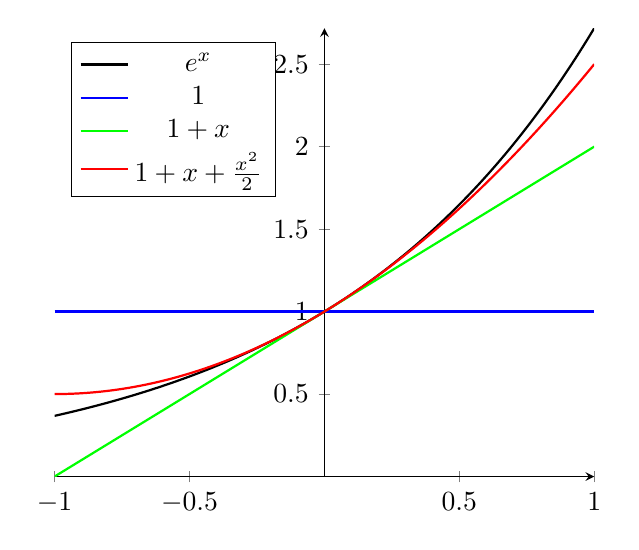
\begin{tikzpicture}
   \begin{axis}[
       axis y line = middle,
       axis x line = middle,
       samples     = 200,
       domain      = -1:1,
       unbounded coords=jump,
       legend pos=north west
     ]
    \addplot[black, thick, mark=none] {exp(x)};
	\addplot[blue, thick, mark=none] {1};     
    \addplot[green, thick, mark=none] {1+x};   
	 \addplot[red, thick, mark=none] {1+x+0.5*x^2};   
	 \addlegendentry{$e^x$}
	 \addlegendentry{$1$}
	 \addlegendentry{$1+x$}
	\addlegendentry{$1+x+\frac{x^2}{2}$}	
   \end{axis}
\end{tikzpicture}
 \end{center}
On "observe" que plus le degré augmente, plus la fonction polynômiale se rapproche rapidement de la fonction exponentielle \impo{au voisinage de zéro} car le reste $x^{n}\epsilon(x)$ est une puissance de $n$.\\   
Basée sur cette propriété, les développements limités permettent de trouver plus simplement des limites de fonctions, de calculer des dérivées, de prouver qu'une fonction est intégrable ou non, ou encore d'étudier des positions de courbes par rapport à des tangentes.

\section{Généralités}
Soit f une fonction réel définie sur un intervalle $I$. Soit $a$ est un point de $I$.
\begin{DefinitionProposition}[Développement limité]
On dit que f admet un \defi{développement limité à l'ordre $n$ en $a$} s'il existe des réels $a_0,\dots,a_n$ tels que
$$ f(a+h)=a_0+a_1 h+\dots +a_n h^n+h^n\epsilon(h) \text{ avec }
 \lim _{h\rightarrow 0}\epsilon(h)=0.$$
$a_0+a_1 h+\dots +a_n h^n$ s'appelle la \defi{la partie régulière} du développement limité.\\ 
Si $f$ admet un développement limité à l'ordre $n$ en $a$, celui-ci est unique.
\end{DefinitionProposition}
\begin{Remarque}
De manière équivalente, la notation petit $o$ est plus souvent utilisée :
$$ f(a+h)=a_0+a_1 h+\dots +a_n h^n+o(h^n).$$
\end{Remarque}
\begin{Proposition}[Existence : Formule de Taylor-Young]
Si $f$ est de classe $C^n$,\\
alors $f$ admet un développement limité à l'ordre $n$ en tout point $a\in I$ donné par
$$ f(a+h)=f(a)+f'(a) h+\dots +\frac{f^{(n)}(a)}{n!} h^n+h^n\epsilon(h) \text{ avec }
 \lim _{h\rightarrow 0}\epsilon(h)=0.$$
\end{Proposition}
\begin{Exemple}[Sinus]
La fonction sinus est $C^\infty$. Comme $\sin^{(n)}(x)=\sin (x + n. \pi/2)$, on a
$$\sin x=x-{\frac {x^{3}}{3!}}+{\frac {x^{5}}{5!}}-\cdots +(-1)^{n}{\frac {x^{2n+1}}{(2n+1)!}}+o(x^{2n+2}).$$
\end{Exemple}
\begin{Remarque}[Au voisinage de $0$]
Dans la pratique, on se ramènera toujours à des développements limités en $0$ par le changement de
variable $x=a+h$. \\
Par exemple, la fonction $x\to\frac{\sin(x)}{x-\pi}$ admet un développement limité d'ordre 1 en $\pi$ égale à :
 $$\frac{\sin(x)}{x-\pi}=\frac{\sin(h+\pi)}{h}=\frac{-\sin(h)}{h}\overbrace{=}^{\text{DL en 0 à l'ordre 2}}\frac{-h+o(h^2)}{h}=-1+o(h).$$
\end{Remarque}
\begin{Proposition}[Développements limités usuels]
\begin{itemize}
\item $e^{x}=1+x+{\frac {x^{2}}{2!}}+{\frac {x^{3}}{3!}}+\cdots +{\frac {x^{n}}{n!}}+o(x^{n})$
\item $\frac {1}{1-x}=1+x+x^{2}+x^{3}+\cdots +x^{n}+o(x^{n})$
\item $\frac {1}{1+x}=1-x+x^{2}-x^{3}+\cdots +(-1)^{n}x^{n}+o(x^{n})$
\item $\ln {(1-x)}=-x-{\frac {x^{2}}{2}}-{\frac {x^{3}}{3}}-\cdots -{\frac {x^{n}}{n}}+o(x^{n})$
\item $\ln {(1+x)}=x-{\frac {x^{2}}{2}}+{\frac {x^{3}}{3}}-\cdots +(-1)^{n-1}{\frac {x^{n}}{n}}+o(x^{n})$
\item $\cos x=1-{\frac {x^{2}}{2!}}+{\frac {x^{4}}{4!}}-\cdots +(-1)^{n}{\frac {x^{2n}}{(2n)!}}+o(x^{2n+1})$
\item $\sin x=x-{\frac {x^{3}}{3!}}+{\frac {x^{5}}{5!}}-\cdots +(-1)^{n}{\frac {x^{2n+1}}{(2n+1)!}}+o(x^{2n+2})$
\item $(1+x)^{a}=1+ax+{\frac {a(a-1)}{2!}}x^{2}+{\frac {a(a-1)(a-2)}{3!}}x^{3}+\cdots +{\frac {a(a-1)(a-2)...(a-n+1)}{n!}}x^{n}+o(x^{n})$
\end{itemize}
\end{Proposition}
\section{Opérations}
Soit $f$ et $g$ admettant en $0$ des développements limités à l'ordre $n$ donnés par
$$ f(h)=P(h) + o(h^n) \text{ et } g(h)=Q(h) + o(h^n) \text{ avec }P,Q\in \R_n[X]$$
\begin{Proposition}[Somme]
Alors $f+g$ admet un développement limité en $0$ à l'ordre $n$ donné par
$$(f+g)(h)=(P(h)+Q(h))+o(h^n).$$
\end{Proposition}
\begin{Exemple}
Le développement limité à l'ordre $3$ en $0$ de de la fonction suivante est :
$$ \frac{1}{1-x}-e^x = (1+x+x^2+x^3+o(x^3))-(1+x+\frac{x^2}{2}+\frac{x^3}{6}+o(x^3))=\frac{x^2}{2}+\frac{5x^3}{6}+o(x^3).$$
\end{Exemple}
\begin{Proposition}[Produit]
Alors $f.g$ admet un développement limité en $0$ à l'ordre $n$ donné par
$$(f.g)(h)=R(h)+o(h^n).$$
où $R$ est le polynôme obtenu en ne gardant dans le produit $PQ$ que les termes de degré inférieur ou égal à $n$.
\end{Proposition}
\begin{Exemple}
Le développement limité à l'ordre $3$ en $0$ de la fonction suivante est :
$$ \sin (x) \cos (2x) = \left(x-\frac{x^{3}}{6}+o(x^3)\right)\left(1-\frac{(2x)^2}{2}+\overbrace{o(x^3)}^{\text{même orde}}\right)=x-\frac{13x^3}{6}+o(x^3).$$
\end{Exemple}


\begin{Proposition}[Composition] 
Si $g$ s'annule en $0$,\\
alors $f\circ g$ admet un développement limité à l'ordre $n$ en $0$ donné par
$$f\circ g(h)=R(h)+o(h^n).$$
où $R$ est le polynôme obtenu en ne gardant dans le produit $P\circ Q$ que les termes de degré inférieur ou égal à $n$.
\end{Proposition}
\begin{Exemple}[Développement limité du dénominateur]
Le développement limité à l'ordre $2$ en $0$ de la fonction suivante est :
$$\frac{1}{1 +e^x}=\frac{1}{1+(1+x+x^2+o(x^2))}=\frac{1}{2}\frac{1}{1 + (\frac{x}{2}+\frac{x^2}{2}+o(x^2))}$$ 
$$\frac{1}{1 +e^x}\overbrace{=}^{\frac{1}{1+u}=1-u+u^2 +o(u^2)}1-\left(\frac{x}{2}+\frac{x^2}{2}\right)+\left(\frac{x}{2}+\frac{x^2}{2}\right)^2+o(x^2)=\frac{1}{2}-\frac 1 4 x +o(x^2).$$
\end{Exemple}
\begin{Proposition}[Quotient]
Si $g$ ne s'annule pas en $0$,\\
alors $\frac f g$ admet un développement limité en $0$ à l'ordre $n$ donné par
$$\left(\frac f g \right)(h)=R(h)+o(h^n).$$
où $R$ est le quotient de la division suivant les puissances croissantes de $P$ par $Q$ jusqu'à l'ordre $n$.
\end{Proposition}
\begin{Remarque}
Pour calculer un développement limité sous forme d'un quotient, il est souvent préférable d'utiliser cette méthode : développement limité du dénominateur puis développement limité du produit.  Par exemple,  le développement limité en 0 à l'ordre 3 de la fonction suivante est :
$$\frac{\ln(1+x)}{\sin x}=\frac{x-\frac{x^2}{2}+\frac{x^3}{3}-\frac{x^4}{4}+o(x^4)}{x-\frac{x^3}{6}+o(x^4)}=\frac{1-\frac{x}{2}+\frac{x^2}{3}-o(x^3)}{1-\frac{x^2}{6}+o(x^3)}.$$
On effectue ensuite le développement limité à l'ordre 3 du dénominateur : 
$$\frac{1}{1-\frac{x^2}{6}+o(x^3)}=1+\frac{x^2}{6}+o(x^3).$$
puis le produit  :
$$\frac{\ln(1+x)}{\sin x}= \left(1-\frac{x}{2}+\frac{x^2}{3}-o(x^3)\right) \left(1+\frac{x^2}{6}+o(x^3)\right)= 1-\frac{x}{2}+\frac{x^2}{2}-\frac{x^3}{3}+o(x^3).$$
\end{Remarque}
\begin{Proposition}[Intégration]
Si $f$ est continue sur $I$ avec $F$ une primitive de $f$,\\
Alors $F$ admet un développement limité à l'ordre $n+1$ en $0$ donné par
$$F(h)=F(0)+a_0 h+\frac{a_1}{2}h^2+\dots +\frac{a_n}{(n+1)!}h^{n+1}+o(h^{n+1}).$$
\end{Proposition}
\begin{Exemple}[Quotient]
La fonction $F:x\to \ln(1-x)$ est une primitive de $f:x\to -\frac{1}{1-x}.$ Comme $F(0)=0$ et $\frac {1}{1-x}=1+x+x^{2}+x^{3}+\cdots +x^{n}+o(x^{n})$, on a
$$ \ln(1-x)=-x-{\frac {x^{2}}{2}}-{\frac {x^{3}}{3}}-\cdots -{\frac {x^{n+1}}{n+1}}+o(x^{n+1}).$$
\end{Exemple}
\section{Applications}

\subsection{Étude d'une fonction}
\begin{enumerate}
\item \textit{Calcul de limite d'une fonction} : déterminer la limite en 0 de la fonction $x\to\frac{\sin x}{x}$. On a : 
$$\frac{\sin x}{x}= \frac{x+o(x)}{x}=1+o(1)\xrightarrow[x\to 0]{} 1.$$
\item \textit{Étude locale d'une courbe} : déterminer la tangente au point d'abscisse 0  et démontrer que la tangente traverse la courbe de la fonction : $x\to \frac{1}{1+e^x}$.\\
En utilisant les technique opératoires classiques, on trouve que :
$$\frac{1}{1+e^x}=\frac 1 2 - \frac 1 4 x + \frac{1}{48}x^3+x^3\epsilon(x).$$
Comme $f\in C^2$, par identification avec la formule de Taylor Young, on obtient que $f(0)=\frac 1 x$ et $f'(0)= - \frac 1 4$. Le graphe est donc tangent à la droite d'équation $y=\frac 1 2 - \frac 1 4 x.$
De plus, $$\frac{1}{1+e^x}- (\frac 1 2 - \frac 1 4 x)= x^3\overbrace{\left(\frac{1}{48}+\epsilon(x)\right)}^{\text{positif pour x petit}}.$$
Donc,  pour $x$ petit, cette quantité est positive pour $x>0$, et négative pour $x<0$ : la courbe traverse sa tangente. C'est un point d'inflexion.
\end{enumerate}


\subsection{Étude d'une suite}
\begin{enumerate}
\item \textit{Calcul de limite d'une suite} : déterminer la limite de la suite donnée par $u_n=(1+\frac a n )^n$. On a : 
$$(1+\frac a n )^n = e^{n\ln(1+\frac a n)}\overbrace{=}^{ \ln(1+x)=x+o(x)\text{ avec }x=\frac 1 n }e^{n\left(\frac a n + o(\frac 1 n)\right) }=e^{a+ o(1)} \xrightarrow[n\to\infty]{}  e^a\text{ car exp est continue.}$$
\item \textit{Déterminer un équivalent} : déterminer la limite de la suite $u_n=\frac{\sqrt{n+1}-\sqrt{n}}{n}$. On a :
$$\frac{\sqrt{n+1}-\sqrt{n}}{n} = \frac{\sqrt{1+\frac 1 n}-1}{\sqrt{n}}\overbrace{=}^{ \sqrt{1+x}=1+\frac x 2 +o(x)\text{ avec }x=\frac 1 n}\frac{1+\frac{1}{2n}+o(\frac 1 n) -1}{\sqrt{n}}=\frac{1}{2n^{3/2}}+o\left(\frac{1}{n^{3/2}}\right).$$
Ainsi
$$\frac{\sqrt{n+1}-\sqrt{n}}{n} \sim_{\infty} \frac{1}{2n^{3/2}}.$$
On conclut que la vitesse de convergence de la suite $(u_n)_{n\in\N}$ vers $0$ est de l'ordre de  $\frac{1}{n^{3/2}}$.  A titre d'exercice, donner la vitesse de convergence de la suite $\left((1+\frac a n )^n\right)_{n\in\N}$ vers $e^a$.
\end{enumerate}
\end{document}
